\section{$\rho_1$ is a 4-transposition}

\begin{theorem}
  If $\rho_1$ is a 4-transposition, then a generator can be written as a product of other generators, and thus the generating set is not free, and the group is not a sggi.
\end{theorem}

\begin{proof}

\paragraph{}
Let's draw a graph with all edges of the 4-transposition $\rho_1$.

\begin{figure}[H]
  \begin{center}
    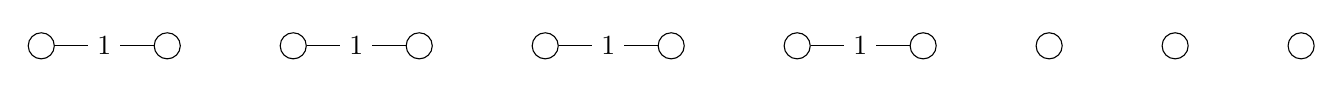
\begin{tikzpicture}[scale=.8]

      \begin{scope}[every node/.style={circle,draw}]
        \node (1)  at (0,0)  {};
        \node (2)  at (2,0)  {};
        \node (3)  at (4,0)  {};
        \node (4)  at (6,0)  {};
        \node (5)  at (8,0)  {};
        \node (6)  at (10,0)  {};
        \node (7)  at (12,0)  {};
        \node (8)  at (14,0)  {};
        \node (9)  at (16,0)  {};
        \node (10) at (18,0)  {};
        \node (11) at (20,0) {};
      \end{scope}

      \begin{scope}[every node/.style={fill=white}]

        \begin{scope}[every edge/.style={draw}]
          \path (1)  edge node {$1$} (2);
          \path (3)  edge node {$1$} (4);
          \path (5)  edge node {$1$} (6);
          \path (7)  edge node {$1$} (8);
        \end{scope}
      \end{scope}

    \end{tikzpicture}
    \caption{}
  \end{center}
\end{figure}

\paragraph{}
This transposition must commute with $\rho_3$ and $\rho_4$. There are three possibilities to place the two $\rho_4$ edges: building an alternating square, doubling one edge a linking two fixed points or doubling two edges.

\subsection{The alternating square}

\begin{figure}[H]
  \begin{center}
    \begin{tikzpicture}[scale=.8]

      \begin{scope}[every node/.style={circle,draw}]
        \node (1)  at (0,2)  {};
        \node (2)  at (0,0)  {};
        \node (3)  at (2,2)  {};
        \node (4)  at (2,0)  {};
        \node (5)  at (4,0)  {};
        \node (6)  at (6,0)  {};
        \node (7)  at (8,0)  {};
        \node (8)  at (10,0)  {};
        \node (9)  at (12,0)  {};
        \node (10) at (14,0)  {};
        \node (11) at (16,0) {};
      \end{scope}

      \begin{scope}[every node/.style={fill=white}]

        \begin{scope}[every edge/.style={draw}]
          \path (1)  edge node {$1$} (2);
          \path (3)  edge node {$1$} (4);
          \path (5)  edge node {$1$} (6);
          \path (7)  edge node {$1$} (8);
          \path (1)  edge node {$4$} (3);
          \path (2)  edge node {$4$} (4);
        \end{scope}
      \end{scope}

    \end{tikzpicture}
    \caption{}
  \end{center}
\end{figure}

\paragraph{}
If $\rho_4$ forms an alternating square with $\rho_1$, it must be adjacent to an other alternating square $[\rho_1, \rho_3]$ ($[\rho_2, \rho_4]$ is not possible because $\rho_4$ is a 2-transposition). The sequence of squares cannot be extended to the right because two extra alternating squares are needed. There is only one remaining $\rho_1$ edge, therefore it is not possible to continue linearly. But a rotation pattern cannot be placed, so it is impossible.

\paragraph{}
If the sequence is extended to the left, the last $\rho_1$ edge and two $\rho_3$ edges would be used. At the end only 2 $\rho_0$ edges and 2 or 4 $\rho_2$ edges remain but they cannot form a connected graph.

\paragraph{}
The sequence of alternating squares must therefore be of length 2. Those squares must be linked to the rest of the graph by a $\rho_2$ edge.

\begin{figure}[H]
  \begin{center}
    \begin{tikzpicture}[scale=.8]

      \begin{scope}[every node/.style={circle,draw}]
        \node (1)  at (0,2)  {};
        \node (2)  at (0,0)  {};
        \node (3)  at (2,2)  {};
        \node (4)  at (2,0)  {};
        \node (5)  at (4,2)  {};
        \node (6)  at (4,0)  {};
        \node (7)  at (6,0)  {};
        \node (8)  at (8,0)  {};
        \node (9)  at (10,0)  {};
        \node (10) at (12,0)  {};
        \node (11) at (14,0) {};
      \end{scope}

      \begin{scope}[every node/.style={fill=white}]

        \begin{scope}[every edge/.style={draw}]
          \path (1)  edge node {$1$} (2);
          \path (3)  edge node {$1$} (4);
          \path (5)  edge node {$1$} (6);
          \path (7)  edge node {$1$} (8);
          \path (3)  edge node {$3$} (5);
          \path (4)  edge node {$3$} (6);
          \path (1)  edge node {$4$} (3);
          \path (2)  edge node {$4$} (4);
        \end{scope}
      \end{scope}

    \end{tikzpicture}
    \caption{}
  \end{center}
\end{figure}


\paragraph{}
By Lemma~\ref{adjacent-must-not-commute} $\rho_0$ and $\rho_1$ must not commute. Thus a $\rho_0$ edge must share a vertex with a $\rho_1$ edge, otherwise $\rho_0$ and $\rho_1$ would commute.

\paragraph{}
By Lemma~\ref{0-4-no-share}, the edges of involutions $\rho_0$ and $\rho_4$ cannot share a vertex. So the $\rho_0$ edge cannot be linked to the first 4 vertices. They cannot be connected thus to the 5th and 6th vertices because it would form an alternating square but it was proved that the sequence cannot be extended.

\paragraph{}
Thus, a $\rho_0$ edge must link the extremity of the single $\rho_1$ edge to a fixed point. The other $\rho_0$ edge must link the two fixed points because if the other extremity of the single $\rho_1$ edge is used, it is not possible to connect the formed component.

\begin{figure}[H]
  \begin{center}
    \begin{tikzpicture}[scale=.8]

      \begin{scope}[every node/.style={circle,draw}]
        \node (1)  at (0,2)  {};
        \node (2)  at (0,0)  {};
        \node (3)  at (2,2)  {};
        \node (4)  at (2,0)  {};
        \node (5)  at (4,2)  {};
        \node (6)  at (4,0)  {};
        \node (7)  at (6,0)  {};
        \node (8)  at (8,0)  {};
        \node (9)  at (10,0)  {};
        \node (10) at (12,0)  {};
        \node (11) at (14,0) {};
      \end{scope}

      \begin{scope}[every node/.style={fill=white}]

        \begin{scope}[every edge/.style={draw}]
          \path (8)  edge node {$0$} (9);
          \path (10)  edge node {$0$} (11);
          \path (1)  edge node {$1$} (2);
          \path (3)  edge node {$1$} (4);
          \path (5)  edge node {$1$} (6);
          \path (7)  edge node {$1$} (8);
          \path (3)  edge node {$3$} (5);
          \path (4)  edge node {$3$} (6);
          \path (1)  edge node {$4$} (3);
          \path (2)  edge node {$4$} (4);
        \end{scope}
      \end{scope}

    \end{tikzpicture}
    \caption{}
  \end{center}
\end{figure}

\paragraph{}
The two alternating squares can only be linked by a $\rho_2$ edge. This edge must be linked to the $\rho_1$ component because it is not possible to continue the sequence.

\begin{figure}[H]
  \begin{center}
    \begin{tikzpicture}[scale=.8]

      \begin{scope}[every node/.style={circle,draw}]
        \node (1)  at (0,2)  {};
        \node (2)  at (0,0)  {};
        \node (3)  at (2,2)  {};
        \node (4)  at (2,0)  {};
        \node (5)  at (4,2)  {};
        \node (6)  at (4,0)  {};
        \node (7)  at (6,0)  {};
        \node (8)  at (8,0)  {};
        \node (9)  at (10,0)  {};
        \node (10) at (12,0)  {};
        \node (11) at (14,0) {};
      \end{scope}

      \begin{scope}[every node/.style={fill=white}]

        \begin{scope}[every edge/.style={draw}]
          \path (8)  edge node {$0$} (9);
          \path (10)  edge node {$0$} (11);
          \path (1)  edge node {$1$} (2);
          \path (3)  edge node {$1$} (4);
          \path (5)  edge node {$1$} (6);
          \path (7)  edge node {$1$} (8);
          \path (6)  edge node {$2$} (7);
          \path (3)  edge node {$3$} (5);
          \path (4)  edge node {$3$} (6);
          \path (1)  edge node {$4$} (3);
          \path (2)  edge node {$4$} (4);
        \end{scope}
      \end{scope}

    \end{tikzpicture}
    \caption{}
  \end{center}
\end{figure}

\paragraph{}
All $\rho_1$ edges have been used, they cannot be used to link the single $\rho_0$. Therefore it is necessary to use an alternating square to connect it. But this alternating square must be connected to a single edge. Therefore the difference between the indices of the edges must be 2. The vertical edges of the square must therefore be $\rho_2$.

\begin{figure}[H]
  \begin{center}
    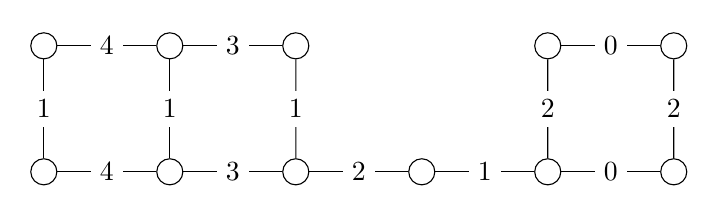
\begin{tikzpicture}[scale=.8]

      \begin{scope}[every node/.style={circle,draw}]
        \node (1)  at (0,2)  {};
        \node (2)  at (0,0)  {};
        \node (3)  at (2,2)  {};
        \node (4)  at (2,0)  {};
        \node (5)  at (4,2)  {};
        \node (6)  at (4,0)  {};
        \node (7)  at (6,0)  {};
        \node (8)  at (8,2)  {};
        \node (9)  at (8,0)  {};
        \node (10) at (10,2)  {};
        \node (11) at (10,0) {};
      \end{scope}

      \begin{scope}[every node/.style={fill=white}]

        \begin{scope}[every edge/.style={draw}]
          \path (9)  edge node {$0$} (11);
          \path (8)  edge node {$0$} (10);
          \path (1)  edge node {$1$} (2);
          \path (3)  edge node {$1$} (4);
          \path (5)  edge node {$1$} (6);
          \path (7)  edge node {$1$} (9);
          \path (6)  edge node {$2$} (7);
          \path (8)  edge node {$2$} (9);
          \path (10) edge node {$2$} (11);
          \path (3)  edge node {$3$} (5);
          \path (4)  edge node {$3$} (6);
          \path (1)  edge node {$4$} (3);
          \path (2)  edge node {$4$} (4);
        \end{scope}
      \end{scope}

    \end{tikzpicture}
    \caption{}
  \end{center}
\end{figure}

\paragraph{}
There are only 3 $\rho_2$ edges on this graph. A last one must be added to restore parity. There are only two places possible: double any of the $\rho_4$ edge. That gives 2 graphs:

\begin{figure}[H]
  \begin{center}
    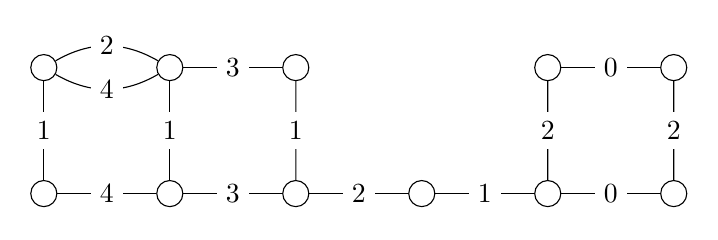
\begin{tikzpicture}[scale=.8]

      \begin{scope}[every node/.style={circle,draw}]
        \node (1)  at (0,2)  {};
        \node (2)  at (0,0)  {};
        \node (3)  at (2,2)  {};
        \node (4)  at (2,0)  {};
        \node (5)  at (4,2)  {};
        \node (6)  at (4,0)  {};
        \node (7)  at (6,0)  {};
        \node (8)  at (8,2)  {};
        \node (9)  at (8,0)  {};
        \node (10) at (10,2)  {};
        \node (11) at (10,0) {};
      \end{scope}

      \begin{scope}[every node/.style={fill=white}]

        \begin{scope}[every edge/.style={draw}]
          \path (9)  edge node {$0$} (11);
          \path (8)  edge node {$0$} (10);
          \path (1)  edge node {$1$} (2);
          \path (3)  edge node {$1$} (4);
          \path (5)  edge node {$1$} (6);
          \path (7)  edge node {$1$} (9);
          \path (1)  edge[bend left=30] node {$2$} (3);
          \path (6)  edge node {$2$} (7);
          \path (8)  edge node {$2$} (9);
          \path (10) edge node {$2$} (11);
          \path (3)  edge node {$3$} (5);
          \path (4)  edge node {$3$} (6);
          \path (1)  edge[bend right=30] node {$4$} (3);
          \path (2)  edge node {$4$} (4);
        \end{scope}
      \end{scope}

    \end{tikzpicture}
    \caption{}
  \end{center}
\end{figure}

\begin{figure}[H]
  \begin{center}
    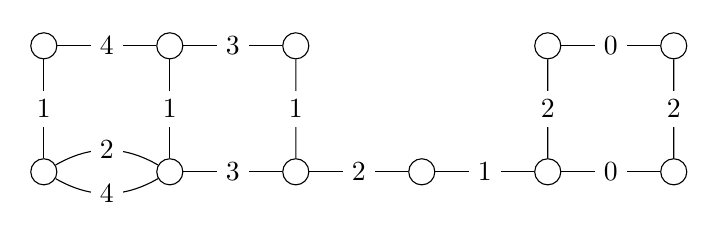
\begin{tikzpicture}[scale=.8]

      \begin{scope}[every node/.style={circle,draw}]
        \node (1)  at (0,2)  {};
        \node (2)  at (0,0)  {};
        \node (3)  at (2,2)  {};
        \node (4)  at (2,0)  {};
        \node (5)  at (4,2)  {};
        \node (6)  at (4,0)  {};
        \node (7)  at (6,0)  {};
        \node (8)  at (8,2)  {};
        \node (9)  at (8,0)  {};
        \node (10) at (10,2)  {};
        \node (11) at (10,0) {};
      \end{scope}

      \begin{scope}[every node/.style={fill=white}]

        \begin{scope}[every edge/.style={draw}]
          \path (9)  edge node {$0$} (11);
          \path (8)  edge node {$0$} (10);
          \path (1)  edge node {$1$} (2);
          \path (3)  edge node {$1$} (4);
          \path (5)  edge node {$1$} (6);
          \path (7)  edge node {$1$} (9);
          \path (2)  edge[bend left=30] node {$2$} (4);
          \path (6)  edge node {$2$} (7);
          \path (8)  edge node {$2$} (9);
          \path (10) edge node {$2$} (11);
          \path (3)  edge node {$3$} (5);
          \path (4)  edge node {$3$} (6);
          \path (1)  edge node {$4$} (3);
          \path (2)  edge[bend right=30] node {$4$} (4);
        \end{scope}
      \end{scope}

    \end{tikzpicture}
    \caption{}
  \end{center}
\end{figure}

\paragraph{}
Those graphs are valid graphs but $\rho_3$ is a 2-transposition. This involution can be extended to a 4-transposition. There are only two possible positions for extra $\rho_3$ edges: double the left $\rho_1$ edge and the upper $\rho_0$ edge. That creates two other graphs:

\begin{figure}[H]
  \begin{center}
    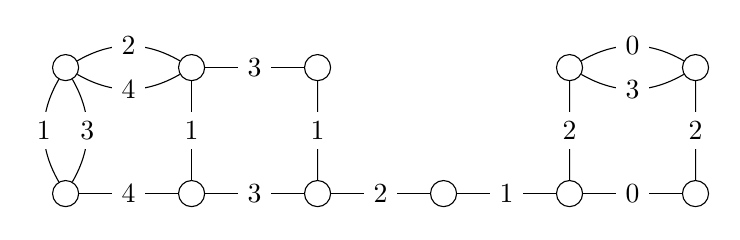
\begin{tikzpicture}[scale=.8]

      \begin{scope}[every node/.style={circle,draw}]
        \node (1)  at (0,2)  {};
        \node (2)  at (0,0)  {};
        \node (3)  at (2,2)  {};
        \node (4)  at (2,0)  {};
        \node (5)  at (4,2)  {};
        \node (6)  at (4,0)  {};
        \node (7)  at (6,0)  {};
        \node (8)  at (8,2)  {};
        \node (9)  at (8,0)  {};
        \node (10) at (10,2)  {};
        \node (11) at (10,0) {};
      \end{scope}

      \begin{scope}[every node/.style={fill=white}]

        \begin{scope}[every edge/.style={draw}]
          \path (9)  edge node {$0$} (11);
          \path (8)  edge[bend left=30] node {$0$} (10);
          \path (1)  edge[bend right=30] node {$1$} (2);
          \path (3)  edge node {$1$} (4);
          \path (5)  edge node {$1$} (6);
          \path (7)  edge node {$1$} (9);
          \path (1)  edge[bend left=30] node {$2$} (3);
          \path (6)  edge node {$2$} (7);
          \path (8)  edge node {$2$} (9);
          \path (10) edge node {$2$} (11);
          \path (1)  edge[bend left=30] node {$3$} (2);
          \path (3)  edge node {$3$} (5);
          \path (4)  edge node {$3$} (6);
          \path (8)  edge[bend right=30] node {$3$} (10);
          \path (1)  edge[bend right=30] node {$4$} (3);
          \path (2)  edge node {$4$} (4);
        \end{scope}
      \end{scope}

    \end{tikzpicture}
    \caption{}
  \end{center}
\end{figure}

\begin{figure}[H]
  \begin{center}
    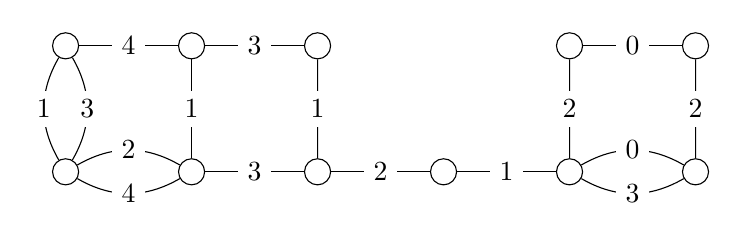
\begin{tikzpicture}[scale=.8]

      \begin{scope}[every node/.style={circle,draw}]
        \node (1)  at (0,2)  {};
        \node (2)  at (0,0)  {};
        \node (3)  at (2,2)  {};
        \node (4)  at (2,0)  {};
        \node (5)  at (4,2)  {};
        \node (6)  at (4,0)  {};
        \node (7)  at (6,0)  {};
        \node (8)  at (8,2)  {};
        \node (9)  at (8,0)  {};
        \node (10) at (10,2)  {};
        \node (11) at (10,0) {};
      \end{scope}

      \begin{scope}[every node/.style={fill=white}]

        \begin{scope}[every edge/.style={draw}]
          \path (9)  edge[bend left=30] node {$0$} (11);
          \path (8)  edge node {$0$} (10);
          \path (1)  edge[bend right=30] node {$1$} (2);
          \path (3)  edge node {$1$} (4);
          \path (5)  edge node {$1$} (6);
          \path (7)  edge node {$1$} (9);
          \path (2)  edge[bend left=30] node {$2$} (4);
          \path (6)  edge node {$2$} (7);
          \path (8)  edge node {$2$} (9);
          \path (10) edge node {$2$} (11);
          \path (1)  edge[bend left=30] node {$3$} (2);
          \path (3)  edge node {$3$} (5);
          \path (4)  edge node {$3$} (6);
          \path (9)  edge[bend right=30] node {$3$} (11);
          \path (1)  edge node {$4$} (3);
          \path (2)  edge[bend right=30] node {$4$} (4);
        \end{scope}
      \end{scope}

    \end{tikzpicture}
    \caption{}
  \end{center}
\end{figure}

\paragraph{}
Let's remove all edges from involutions $\rho_0$ and $\rho_3$:

\begin{figure}[H]
  \begin{center}
    \begin{tikzpicture}[scale=.8]

      \begin{scope}[every node/.style={circle,draw}]
        \node (1)  at (0,2)  {};
        \node (2)  at (0,0)  {};
        \node (3)  at (2,2)  {};
        \node (4)  at (2,0)  {};
        \node (5)  at (6,0)  {};
        \node (6)  at (4,0)  {};
        \node (7)  at (8,0)  {};
        \node (8)  at (10,0)  {};
        \node (9)  at (12,0)  {};
        \node (10) at (14,0)  {};
        \node (11) at (16,0) {};
      \end{scope}

      \begin{scope}[every node/.style={fill=white}]

        \begin{scope}[every edge/.style={draw}]
          \path (1)  edge node {$1$} (2);
          \path (3)  edge node {$1$} (4);
          \path (5)  edge node {$1$} (6);
          \path (7)  edge node {$1$} (8);
          \path (1)  edge[bend left=30] node {$2$} (3);
          \path (5)  edge node {$2$} (7);
          \path (8)  edge node {$2$} (9);
          \path (10) edge node {$2$} (11);
          \path (1)  edge[bend right=30] node {$4$} (3);
          \path (2)  edge node {$4$} (4);
        \end{scope}
      \end{scope}

    \end{tikzpicture}
    \caption{}
  \end{center}
\end{figure}

\paragraph{}
Now it can easily be seen that $\rho_4 = (\rho_1 \rho_2)^{10}$. Thus none of those four graphs have a free set of generators and so none of then are sggis.

\section{A double edge and a single edge between two fixed points}

\paragraph{}
The second possibility is having a double edge $(\rho_0, \rho_4)$. By Lemma~\ref{todo}, an alternating square must be placed next to it in order to allow it to be connected to the rest of the graph. There are possibilities for the alternating square: $[\rho_1, \rho_3]$ or $[\rho_2, \rho_4]$.
\subsection{Alternating square $[\rho_1, \rho_3]$}

\begin{figure}[H]
  \begin{center}
    \begin{tikzpicture}[scale=.8]

      \begin{scope}[every node/.style={circle,draw}]
        \node (1)  at (0,2)  {};
        \node (2)  at (0,0)  {};
        \node (3)  at (2,2)  {};
        \node (4)  at (2,0)  {};
        \node (5)  at (4,0)  {};
        \node (6)  at (6,0)  {};
        \node (7)  at (8,0)  {};
        \node (8)  at (10,0)  {};
        \node (9)  at (12,0)  {};
        \node (10) at (14,0)  {};
        \node (11) at (16,0) {};
      \end{scope}

      \begin{scope}[every node/.style={fill=white}]

        \begin{scope}[every edge/.style={draw}]
          \path (1)  edge[bend right=30] node {$1$} (2);
          \path (3)  edge node {$1$} (4);
          \path (5)  edge node {$1$} (6);
          \path (7)  edge node {$1$} (8);
          \path (1)  edge node {$3$} (3);
          \path (2)  edge node {$3$} (4);
          \path (1)  edge[bend left=30] node {$4$} (2);
        \end{scope}
      \end{scope}

    \end{tikzpicture}
    \caption{}
  \end{center}
\end{figure}

\paragraph{}
By lemma~\ref{todo}, $\rho_0$ and $\rho_1$ must not commute. A $\rho_0$ edge must thus be connected to at least one $\rho_1$ edge. So at least one $\rho_1$ edge must not be part of an alternating square of which $\rho_0$ does not belong.

\paragraph{}
This alternating square cannot be linked by another alternating square on the right because it will need two alternating squares on the right if the value of the vertical edges is not changed. But that uses all $\rho_1$ in alternating squares, which is not possible by the previous statement.

\paragraph{}
The values of the vertical edges must therefore be changed. The horizontal edges of the second square must be $\rho_2$ because the involutions must be adjacent to $\rho_3$ and there is not enough $\rho_4$ edges. Then the new value for vertical edge must be adjacent to $\rho_3$. $\rho_2$ is impossible because it is already used for the horizontal edges. The only remaining possibility is $\rho_4$ but there are no enough remaining edges.

\paragraph{}
If an alternating square is attached on the left, it must be $[\rho_2, \rho_4]$.

\begin{figure}[H]
  \begin{center}
    \begin{tikzpicture}[scale=.8]

      \begin{scope}[every node/.style={circle,draw}]
        \node (1)  at (0,2)  {};
        \node (2)  at (0,0)  {};
        \node (3)  at (2,2)  {};
        \node (4)  at (2,0)  {};
        \node (5)  at (4,0)  {};
        \node (6)  at (6,0)  {};
        \node (7)  at (8,0)  {};
        \node (8)  at (10,0)  {};
        \node (9)  at (-2,2)  {};
        \node (10) at (-2,0)  {};
        \node (11) at (12,0) {};
      \end{scope}

      \begin{scope}[every node/.style={fill=white}]

        \begin{scope}[every edge/.style={draw}]
          \path (1)  edge[bend right=30] node {$1$} (2);
          \path (3)  edge node {$1$} (4);
          \path (5)  edge node {$1$} (6);
          \path (7)  edge node {$1$} (8);
          \path (1)  edge node {$2$} (9);
          \path (2)  edge node {$2$} (10);
          \path (1)  edge node {$3$} (3);
          \path (2)  edge node {$3$} (4);
          \path (1)  edge[bend left=30] node {$4$} (2);
          \path (9)  edge node {$4$} (10);
        \end{scope}
      \end{scope}

    \end{tikzpicture}
    \caption{}
  \end{center}
\end{figure}

\paragraph{}
The two $\rho_0$ edges cannot be placed on any vertex of the left component. If the fixed point is not used to connect the $\rho_0$ edges, the two $\rho_1$ edges must be linked together twice and thus build an alternating square. Then $\rho_0$ and $\rho_1$ commute and that is impossible. Thus the fixed point must be connected by $\rho_0$.

\paragraph{}
The first $\rho_0$ edge must connect the fixed point to a $\rho_1$ edge and the second must connect the two $\rho_1$ edges together.

\begin{figure}[H]
  \begin{center}
    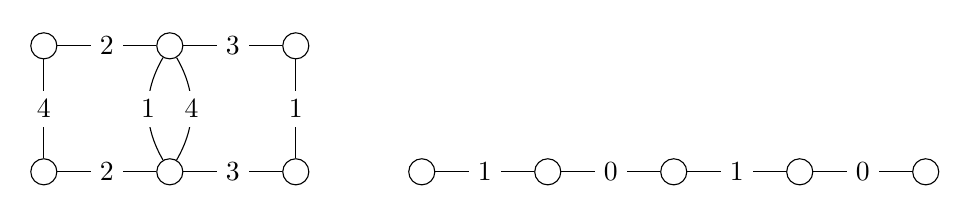
\begin{tikzpicture}[scale=.8]

      \begin{scope}[every node/.style={circle,draw}]
        \node (1)  at (0,2)  {};
        \node (2)  at (0,0)  {};
        \node (3)  at (2,2)  {};
        \node (4)  at (2,0)  {};
        \node (5)  at (4,0)  {};
        \node (6)  at (6,0)  {};
        \node (7)  at (8,0)  {};
        \node (8)  at (10,0)  {};
        \node (9)  at (-2,2)  {};
        \node (10) at (-2,0)  {};
        \node (11) at (12,0) {};
      \end{scope}

      \begin{scope}[every node/.style={fill=white}]

        \begin{scope}[every edge/.style={draw}]
          \path (6)  edge node {$0$} (7);
          \path (8)  edge node {$0$} (11);
          \path (1)  edge[bend right=30] node {$1$} (2);
          \path (3)  edge node {$1$} (4);
          \path (5)  edge node {$1$} (6);
          \path (7)  edge node {$1$} (8);
          \path (1)  edge node {$2$} (9);
          \path (2)  edge node {$2$} (10);
          \path (1)  edge node {$3$} (3);
          \path (2)  edge node {$3$} (4);
          \path (1)  edge[bend left=30] node {$4$} (2);
          \path (9)  edge node {$4$} (10);
        \end{scope}
      \end{scope}

    \end{tikzpicture}
    \caption{}
  \end{center}
\end{figure}

\paragraph{}
Two components must be linked by a $\rho_2$ edge. But the total number of $\rho_2$ edges becomes odd. Another $\rho_2$ must thus be placed. The only possibilities are to double a $\rho_0$ edge. There are two possible graphs:

\begin{figure}[H]
  \begin{center}
    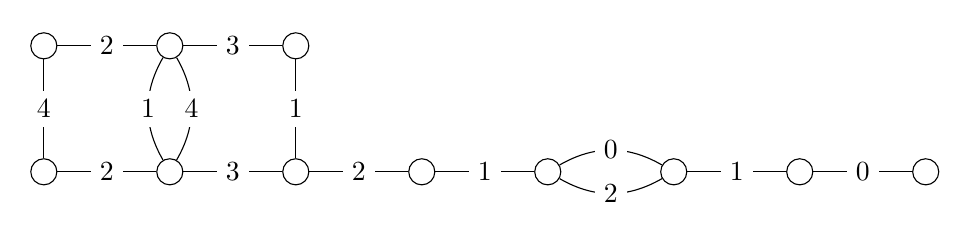
\begin{tikzpicture}[scale=.8]

      \begin{scope}[every node/.style={circle,draw}]
        \node (1)  at (0,2)  {};
        \node (2)  at (0,0)  {};
        \node (3)  at (2,2)  {};
        \node (4)  at (2,0)  {};
        \node (5)  at (4,0)  {};
        \node (6)  at (6,0)  {};
        \node (7)  at (8,0)  {};
        \node (8)  at (10,0)  {};
        \node (9)  at (-2,2)  {};
        \node (10) at (-2,0)  {};
        \node (11) at (12,0) {};
      \end{scope}

      \begin{scope}[every node/.style={fill=white}]

        \begin{scope}[every edge/.style={draw}]
          \path (6)  edge[bend left=30] node {$0$} (7);
          \path (8)  edge node {$0$} (11);
          \path (1)  edge[bend right=30] node {$1$} (2);
          \path (3)  edge node {$1$} (4);
          \path (5)  edge node {$1$} (6);
          \path (7)  edge node {$1$} (8);
          \path (1)  edge node {$2$} (9);
          \path (2)  edge node {$2$} (10);
          \path (4)  edge node {$2$} (5);
          \path (6)  edge[bend right=30] node {$2$} (7);
          \path (1)  edge node {$3$} (3);
          \path (2)  edge node {$3$} (4);
          \path (1)  edge[bend left=30] node {$4$} (2);
          \path (9)  edge node {$4$} (10);
        \end{scope}
      \end{scope}

    \end{tikzpicture}
    \caption{}
  \end{center}
\end{figure}

\begin{figure}[H]
  \begin{center}
    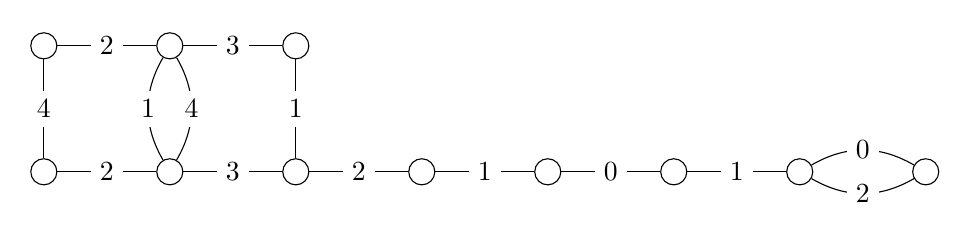
\begin{tikzpicture}[scale=.8]

      \begin{scope}[every node/.style={circle,draw}]
        \node (1)  at (0,2)  {};
        \node (2)  at (0,0)  {};
        \node (3)  at (2,2)  {};
        \node (4)  at (2,0)  {};
        \node (5)  at (4,0)  {};
        \node (6)  at (6,0)  {};
        \node (7)  at (8,0)  {};
        \node (8)  at (10,0)  {};
        \node (9)  at (-2,2)  {};
        \node (10) at (-2,0)  {};
        \node (11) at (12,0) {};
      \end{scope}

      \begin{scope}[every node/.style={fill=white}]

        \begin{scope}[every edge/.style={draw}]
          \path (6)  edge node {$0$} (7);
          \path (8)  edge[bend left=30] node {$0$} (11);
          \path (1)  edge[bend right=30] node {$1$} (2);
          \path (3)  edge node {$1$} (4);
          \path (5)  edge node {$1$} (6);
          \path (7)  edge node {$1$} (8);
          \path (1)  edge node {$2$} (9);
          \path (2)  edge node {$2$} (10);
          \path (4)  edge node {$2$} (5);
          \path (8)  edge[bend right=30] node {$2$} (11);
          \path (1)  edge node {$3$} (3);
          \path (2)  edge node {$3$} (4);
          \path (1)  edge[bend left=30] node {$4$} (2);
          \path (9)  edge node {$4$} (10);
        \end{scope}
      \end{scope}

    \end{tikzpicture}
    \caption{}
  \end{center}
\end{figure}

\paragraph{}
In those graphs, if the $\rho_4$ edge is removed, the generated group is 2-transitive\footnote{TO DO} and thus primitive. By looking at the size of the subgroups, it is possible to deduce that the generated group is $A_{11}$\footnote{Missing the case where no other square are attached}.

\subsection{Alternating square $[\rho_2,\rho_4]$}

\begin{figure}[H]
  \begin{center}
    \begin{tikzpicture}[scale=.8]

      \begin{scope}[every node/.style={circle,draw}]
        \node (1)  at (0,2)  {};
        \node (2)  at (0,0)  {};
        \node (3)  at (2,2)  {};
        \node (4)  at (2,0)  {};
        \node (5)  at (6,0)  {};
        \node (6)  at (4,0)  {};
        \node (7)  at (10,0)  {};
        \node (8)  at (8,0)  {};
        \node (9)  at (12,0)  {};
        \node (10) at (14,0)  {};
        \node (11) at (16,0) {};
      \end{scope}

      \begin{scope}[every node/.style={fill=white}]

        \begin{scope}[every edge/.style={draw}]
          \path (1)  edge[bend right=30] node {$1$} (2);
          \path (5)  edge node {$1$} (6);
          \path (7)  edge node {$1$} (8);
          \path (9)  edge node {$1$} (10);
          \path (1)  edge node {$2$} (3);
          \path (2)  edge node {$2$} (4);
          \path (1)  edge[bend left=30] node {$4$} (2);
          \path (3)  edge node {$4$} (4);
        \end{scope}
      \end{scope}

    \end{tikzpicture}
    \caption{}
  \end{center}
\end{figure}

\paragraph{}
Either two extra alternating squares can be added or this alternating square can be linked to some other component.

\paragraph{}
In the first case, it is impossible to add another alternating square to right of this sequence.

\paragraph{}
The alternating square can however be extended to the left by a $[\rho_1, \rho_3]$ edge but then it can be reduced to the $[\rho_1, \rho_3]$ case.

\paragraph{}
The only remaining possibility is to link to square to the rest of the graph with a single edge. A $\rho_3$ edge must be used. It cannot be connected to a $\rho_1$ edge an alternating square should be built but that is impossible. The only possibility is to link it to the fixed point.

\begin{figure}[H]
  \begin{center}
    \begin{tikzpicture}[scale=.8]

      \begin{scope}[every node/.style={circle,draw}]
        \node (1)  at (0,2)  {};
        \node (2)  at (0,0)  {};
        \node (3)  at (2,2)  {};
        \node (4)  at (2,0)  {};
        \node (5)  at (8,0)  {};
        \node (6)  at (6,0)  {};
        \node (7)  at (12,0)  {};
        \node (8)  at (10,0)  {};
        \node (9)  at (14,0)  {};
        \node (10) at (16,0)  {};
        \node (11) at (4,0) {};
      \end{scope}

      \begin{scope}[every node/.style={fill=white}]

        \begin{scope}[every edge/.style={draw}]
          \path (1)  edge[bend right=30] node {$1$} (2);
          \path (5)  edge node {$1$} (6);
          \path (7)  edge node {$1$} (8);
          \path (9)  edge node {$1$} (10);
          \path (1)  edge node {$2$} (3);
          \path (2)  edge node {$2$} (4);
          \path (4)  edge node {$3$} (11);
          \path (1)  edge[bend left=30] node {$4$} (2);
          \path (3)  edge node {$4$} (4);
        \end{scope}
      \end{scope}

    \end{tikzpicture}
    \caption{}
  \end{center}
\end{figure}

\paragraph{}
Two $\rho_0$ edges must still be placed and they must not commute with $\rho_1$. Thus at least one edge must link two $\rho_1$ involutions. And the other $\rho_0$ edge must link the two other $\rho_1$ edges.

\begin{figure}[H]
  \begin{center}
    \begin{tikzpicture}[scale=.8]

      \begin{scope}[every node/.style={circle,draw}]
        \node (1)  at (0,2)  {};
        \node (2)  at (0,0)  {};
        \node (3)  at (2,2)  {};
        \node (4)  at (2,0)  {};
        \node (5)  at (8,0)  {};
        \node (6)  at (6,0)  {};
        \node (7)  at (12,0)  {};
        \node (8)  at (10,0)  {};
        \node (9)  at (14,0)  {};
        \node (10) at (16,0)  {};
        \node (11) at (4,0) {};
      \end{scope}

      \begin{scope}[every node/.style={fill=white}]

        \begin{scope}[every edge/.style={draw}]
          \path (5)  edge node {$0$} (8);
          \path (7)  edge node {$0$} (9);
          \path (1)  edge[bend right=30] node {$1$} (2);
          \path (5)  edge node {$1$} (6);
          \path (7)  edge node {$1$} (8);
          \path (9)  edge node {$1$} (10);
          \path (1)  edge node {$2$} (3);
          \path (2)  edge node {$2$} (4);
          \path (4)  edge node {$3$} (11);
          \path (1)  edge[bend left=30] node {$4$} (2);
          \path (3)  edge node {$4$} (4);
        \end{scope}
      \end{scope}

    \end{tikzpicture}
    \caption{}
  \end{center}
\end{figure}

\paragraph{}
Since all $\rho_4$ edge have been used and since no $\rho_2$ can be connected to the alternating square, a $\rho_2$ edge must be used to connect the two components together.

\begin{figure}[H]
  \begin{center}
    \begin{tikzpicture}[scale=.8]

      \begin{scope}[every node/.style={circle,draw}]
        \node (1)  at (0,2)  {};
        \node (2)  at (0,0)  {};
        \node (3)  at (2,2)  {};
        \node (4)  at (2,0)  {};
        \node (5)  at (8,0)  {};
        \node (6)  at (6,0)  {};
        \node (7)  at (12,0)  {};
        \node (8)  at (10,0)  {};
        \node (9)  at (14,0)  {};
        \node (10) at (16,0)  {};
        \node (11) at (4,0) {};
      \end{scope}

      \begin{scope}[every node/.style={fill=white}]

        \begin{scope}[every edge/.style={draw}]
          \path (5)  edge node {$0$} (8);
          \path (7)  edge node {$0$} (9);
          \path (1)  edge[bend right=30] node {$1$} (2);
          \path (5)  edge node {$1$} (6);
          \path (7)  edge node {$1$} (8);
          \path (9)  edge node {$1$} (10);
          \path (1)  edge node {$2$} (3);
          \path (2)  edge node {$2$} (4);
          \path (11)  edge node {$2$} (6);
          \path (4)  edge node {$3$} (11);
          \path (1)  edge[bend left=30] node {$4$} (2);
          \path (3)  edge node {$4$} (4);
        \end{scope}
      \end{scope}

    \end{tikzpicture}
    \caption{}
  \end{center}
\end{figure}

\paragraph{}
The $\rho_3$ involution is currently odd. An extra $\rho_3$ edge must be placed. The only possibility is to triple the double edge. The missing $\rho_2$ edge must then be placed such that a $\rho_0$ edge is doubled. There are two graphs:


\begin{figure}[H]
  \begin{center}
    \begin{tikzpicture}[scale=.8]

      \begin{scope}[every node/.style={circle,draw}]
        \node (1)  at (0,2)  {};
        \node (2)  at (0,0)  {};
        \node (3)  at (2,2)  {};
        \node (4)  at (2,0)  {};
        \node (5)  at (8,0)  {};
        \node (6)  at (6,0)  {};
        \node (7)  at (12,0)  {};
        \node (8)  at (10,0)  {};
        \node (9)  at (14,0)  {};
        \node (10) at (16,0)  {};
        \node (11) at (4,0) {};
      \end{scope}

      \begin{scope}[every node/.style={fill=white}]

        \begin{scope}[every edge/.style={draw}]
          \path (5)  edge[bend left=30] node {$0$} (8);
          \path (7)  edge node {$0$} (9);
          \path (1)  edge[bend right=40] node {$1$} (2);
          \path (5)  edge node {$1$} (6);
          \path (7)  edge node {$1$} (8);
          \path (9)  edge node {$1$} (10);
          \path (1)  edge node {$2$} (3);
          \path (2)  edge node {$2$} (4);
          \path (5)  edge[bend right=30] node {$2$} (8);
          \path (11) edge node {$2$} (6);
          \path (1)  edge node {$3$} (2);
          \path (4)  edge node {$3$} (11);
          \path (1)  edge[bend left=40] node {$4$} (2);
          \path (3)  edge node {$4$} (4);
        \end{scope}
      \end{scope}

    \end{tikzpicture}
    \caption{}
  \end{center}
\end{figure}

\begin{figure}[H]
  \begin{center}
    \begin{tikzpicture}[scale=.8]

      \begin{scope}[every node/.style={circle,draw}]
        \node (1)  at (0,2)  {};
        \node (2)  at (0,0)  {};
        \node (3)  at (2,2)  {};
        \node (4)  at (2,0)  {};
        \node (5)  at (8,0)  {};
        \node (6)  at (6,0)  {};
        \node (7)  at (12,0)  {};
        \node (8)  at (10,0)  {};
        \node (9)  at (14,0)  {};
        \node (10) at (16,0)  {};
        \node (11) at (4,0) {};
      \end{scope}

      \begin{scope}[every node/.style={fill=white}]

        \begin{scope}[every edge/.style={draw}]
          \path (5)  edge node {$0$} (8);
          \path (7)  edge[bend left=30] node {$0$} (9);
          \path (1)  edge[bend right=40] node {$1$} (2);
          \path (5)  edge node {$1$} (6);
          \path (7)  edge node {$1$} (8);
          \path (9)  edge node {$1$} (10);
          \path (1)  edge node {$2$} (3);
          \path (2)  edge node {$2$} (4);
          \path (7)  edge[bend right=30] node {$2$} (9);
          \path (11) edge node {$2$} (6);
          \path (1)  edge node {$3$} (2);
          \path (4)  edge node {$3$} (11);
          \path (1)  edge[bend left=40] node {$4$} (2);
          \path (3)  edge node {$4$} (4);
        \end{scope}
      \end{scope}

    \end{tikzpicture}
    \caption{}
  \end{center}
\end{figure}

\paragraph{}
There are no possibility to convert $\rho_3$ to a 4-transposition in this case.

\paragraph{}
The $\rho_0$ and $\rho_3$ edges can be removed and the obtained graph is the same as those obtained for the alternating square $[\rho_1,\rho_4]$. The consequence are the same: $\rho_4 = (\rho_1\rho_2)^{10}$. The group represented by the previous graphs are therefore not sggi.

\section{Two double edges}

\paragraph{}
The double edges must be contained into alternating squares.

\paragraph{}
If the double edges are placed on the same alternating square, it has already been proved that this does not lead anywhere\footnote{This proof has been deleted}.

\paragraph{}
If the two double edges are place on two different squares, those squares use eight points out of eleven. But it is not possible to place the $\rho_0$ edges such that they do not touch any alternating square.

\end{proof}
